\chapter{JUNO实验能谱分bin策略}
%=====================================================================
在反应堆反中微子振荡分析中，能谱的分bin策略既是统计问题也是物理问题——不同的分箱尺度会改变单个 bin 的统计属性、影响谱形信息的保留程度，并进而影响振荡参数估计的偏差与精度。本部分首先明确两个必须区分的能谱概念：一是探测器层面的重建能谱（reconstructed-energy spectrum），即把沉积能量通过能量响应与重构程序得到的、用于拟合的观测直方图；二是物理层面的反应堆中微子能谱（reactor $\bar\nu_e$ spectrum），即裂变同位素在反应堆中产生的原始入射通量及其模型化表达。两类能谱的分bin选择各有侧重点：重建能谱的分bin决定了观测统计与似然近似的有效性；反应堆能谱的分段决定了模型依赖性与外场约束（如来自 Daya Bay 的近场测量）能否有效抑制谱形不确定性。

具体地，重建能谱在低统计量条件下如果使用过细的分箱，会导致若干边缘箱（尤其是谱尾或窄能区）内事件数过小，从而违背常用高斯近似的前提。当基于高斯近似构造 χ² 或直接套用 Wilks 定理来估计置信区间时，这类近似失效会引入系统性偏差，甚至导致置信区间的覆盖率不正确。相对地，反应堆中微子能谱的分段若过细，所定义的谱形自由度可能超出近点探测器实验（Daya Bay reactor neutrino experiment）提供的约束能力，使得拟合对反应堆模型的依赖性增强，从而在不同模型假设下产生可观的系统误差。因此，分箱策略必须在“保留谱形细节以维持灵敏度”与“避免统计近似失效及模型依赖过强”之间找到平衡点。

为了解决上述矛盾并给出可操作的建议，本部分将采用定量化方法：一方面通过大量 toy-MC 实验评估在不同重建能谱分箱下（从非常细到较粗）振荡参数估计的偏差与覆盖率，比较基于高斯近似（CNP,Pearson）与基于泊松似然的统计量在低统计情形下的表现；另一方面构造两类反应堆谱情形——一个为固定反应堆模型（fiducial spectrum），另一个为包含小幅谱形扰动的变化模型（model variation），在不同反应堆能谱分段尺度下比较拟合的精度与由模型依赖引入的系统误差。通过这种“固定-扰动”对比实验，我们将量化在何种中微子能谱分段尺度下，反应堆模型依赖对关键振荡参数（如 $\Delta m^2$）的影响可被接受，从而给出实验可采纳的分bin建议。
本章研究的成果被江门中微子实验合作组采用，并应用与第一篇物理文章的振荡分析中。本章的组织如下：第1节介绍重建能谱的分bin策略；第二节介绍反应堆能谱的分bin策略。

\section{重建能谱分bin策略与低统计量下太阳振荡参数的测量}
本节讨论在低统计量条件下对太阳中微子振荡参数 $\Delta m^2_{21}$ 和 $\sin^2\theta_{12}$ 的测量。我们首先生成5000个伪实验数据集，振荡参数和系统学参数均取名义值，并同时包含统计涨落和系统误差涨落。然后，我们比较基于高斯近似（CNP,Pearson）与基于泊松似然的统计量在低统计情形下的表现。最后，我们给出在不同重建能谱分bin策略下，太阳振荡参数的偏差与精度。

生成 toy 数据所使用的配置与~\ref{sec:Arrived neutrino spectrum}中相同。特别地，在以下结果中，我们对 Asimov 数据以及伪实验均采用组合的 Pearson–Neyman 统计量 $\chi^2_{\mathrm{CNP}}$，这种选择旨在减小振荡参数估计中的偏差。

最后，在相同的伪实验集合下，我们考察了不同重建能谱分 bin 策略对太阳振荡参数偏差（bias）与测量精度（precision）的影响。通过比较各分 bin 方案下的拟合输出分布、均值偏差与置信区间宽度，能够定量判断在早期低统计阶段采用何种分 bin 策略可在保持统计灵敏度的同时尽量抑制由高斯近似失效或低统计量引起的系统性偏差。
\subsection{Toy MC 研究}

在多个曝光时间下，生成了5000个伪实验数据集。振荡参数和系统学参数均取名义值，并同时包含统计涨落和系统误差涨落。

\begin{figure}[ht]
    \centering
    \begin{subfigure}[t]{0.47\textwidth}
      \centering
      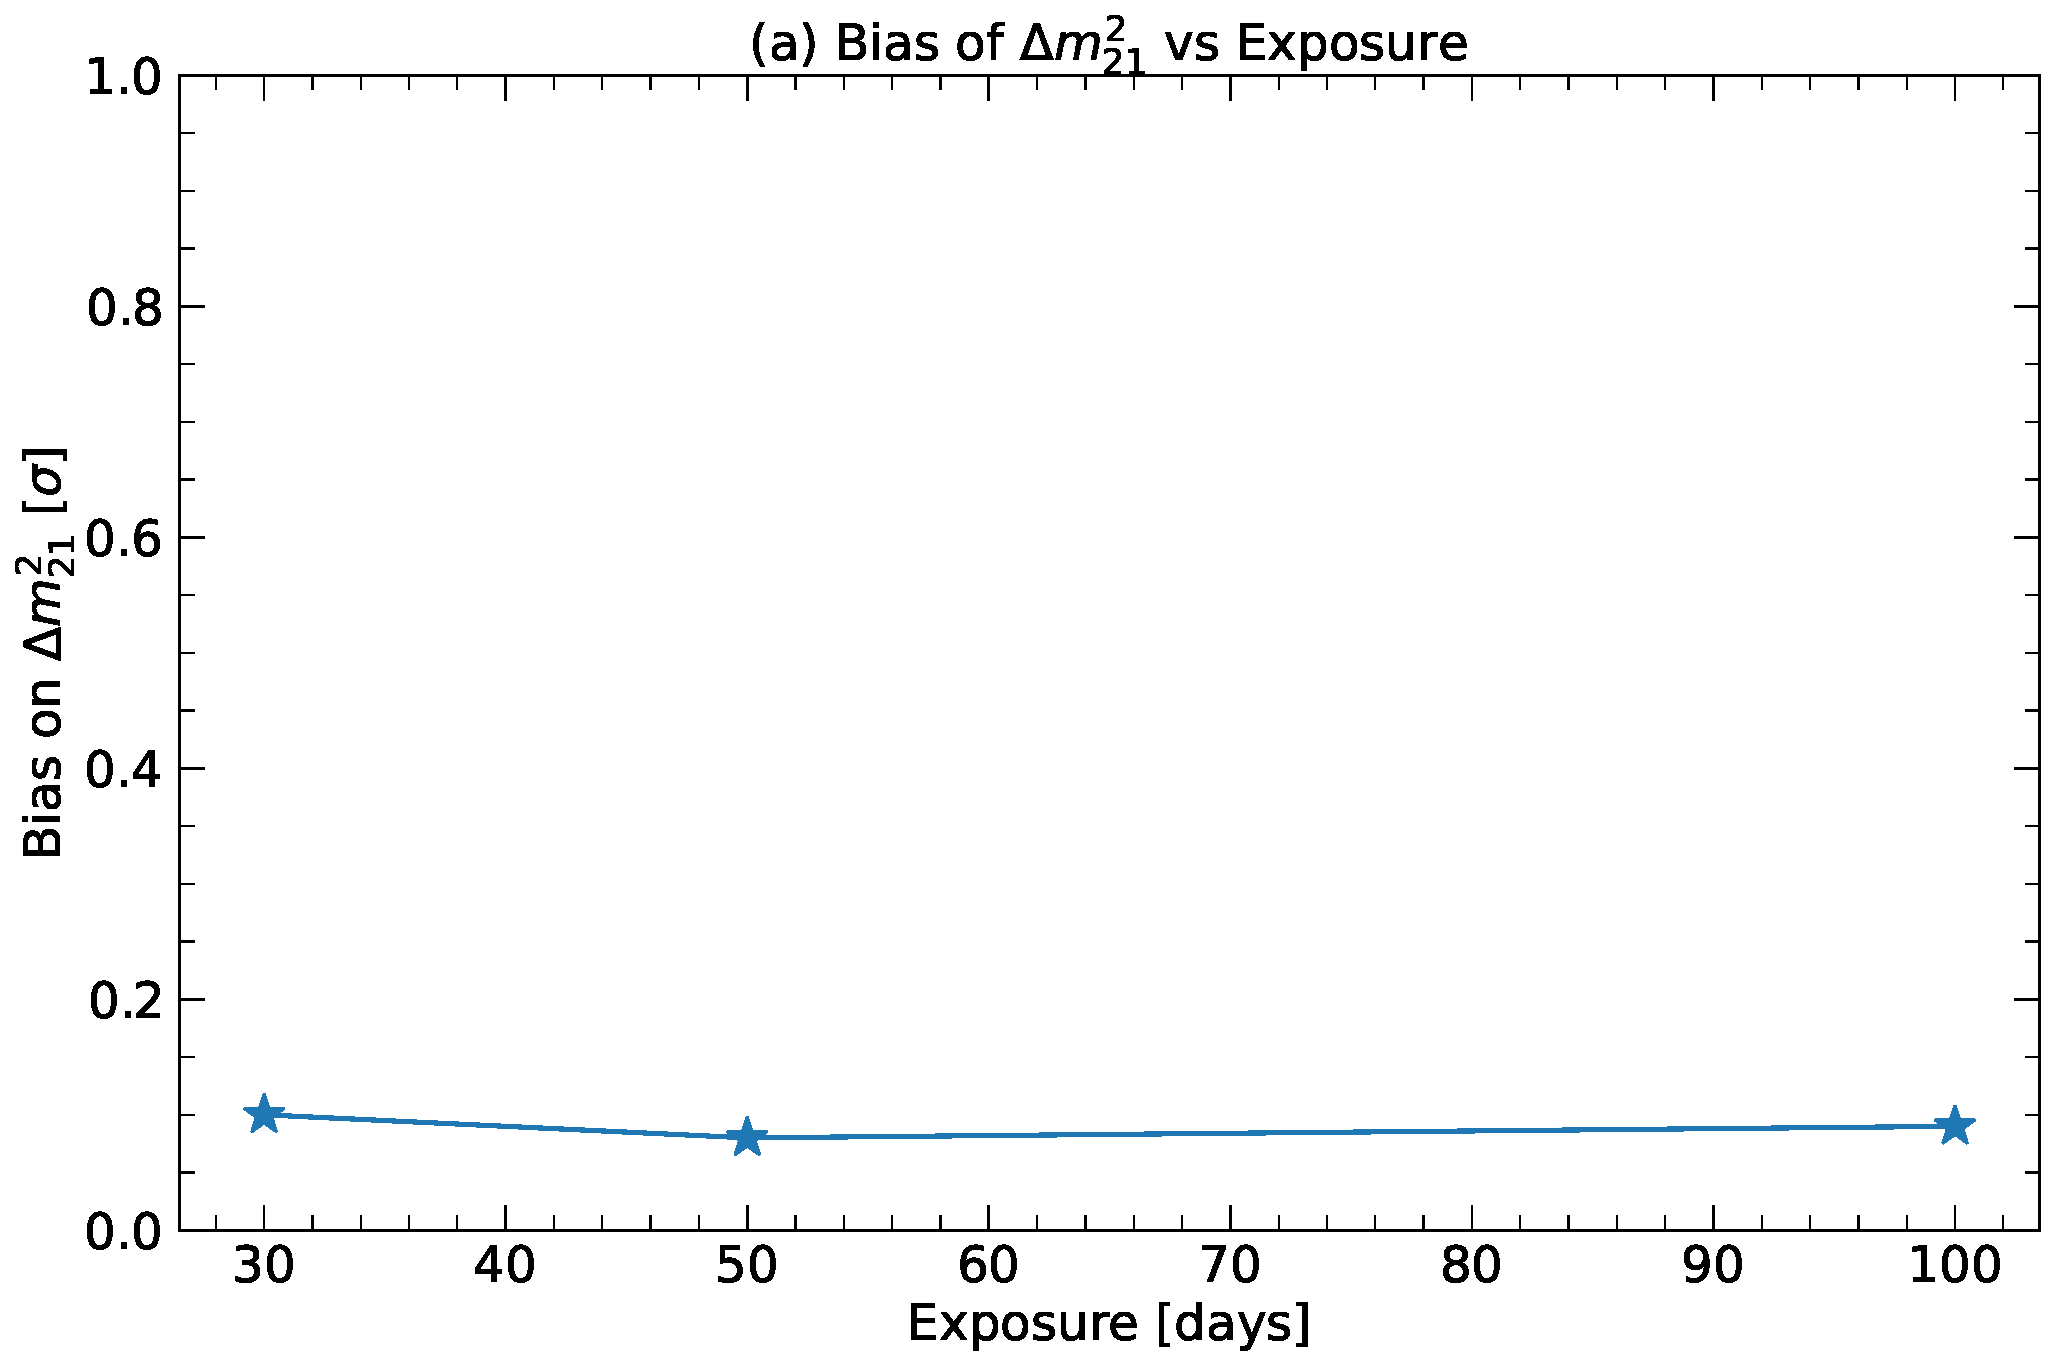
\includegraphics[width=\linewidth]{Img/binning strategy/Bias_of_dm21_vs_exposure.pdf}
      \caption{$\Delta m^2_{21}$ 偏差随时间的变化.}
      \label{fig:dm2_21_bias}
    \end{subfigure}
    \hfill
    \begin{subfigure}[t]{0.47\textwidth}
      \centering
      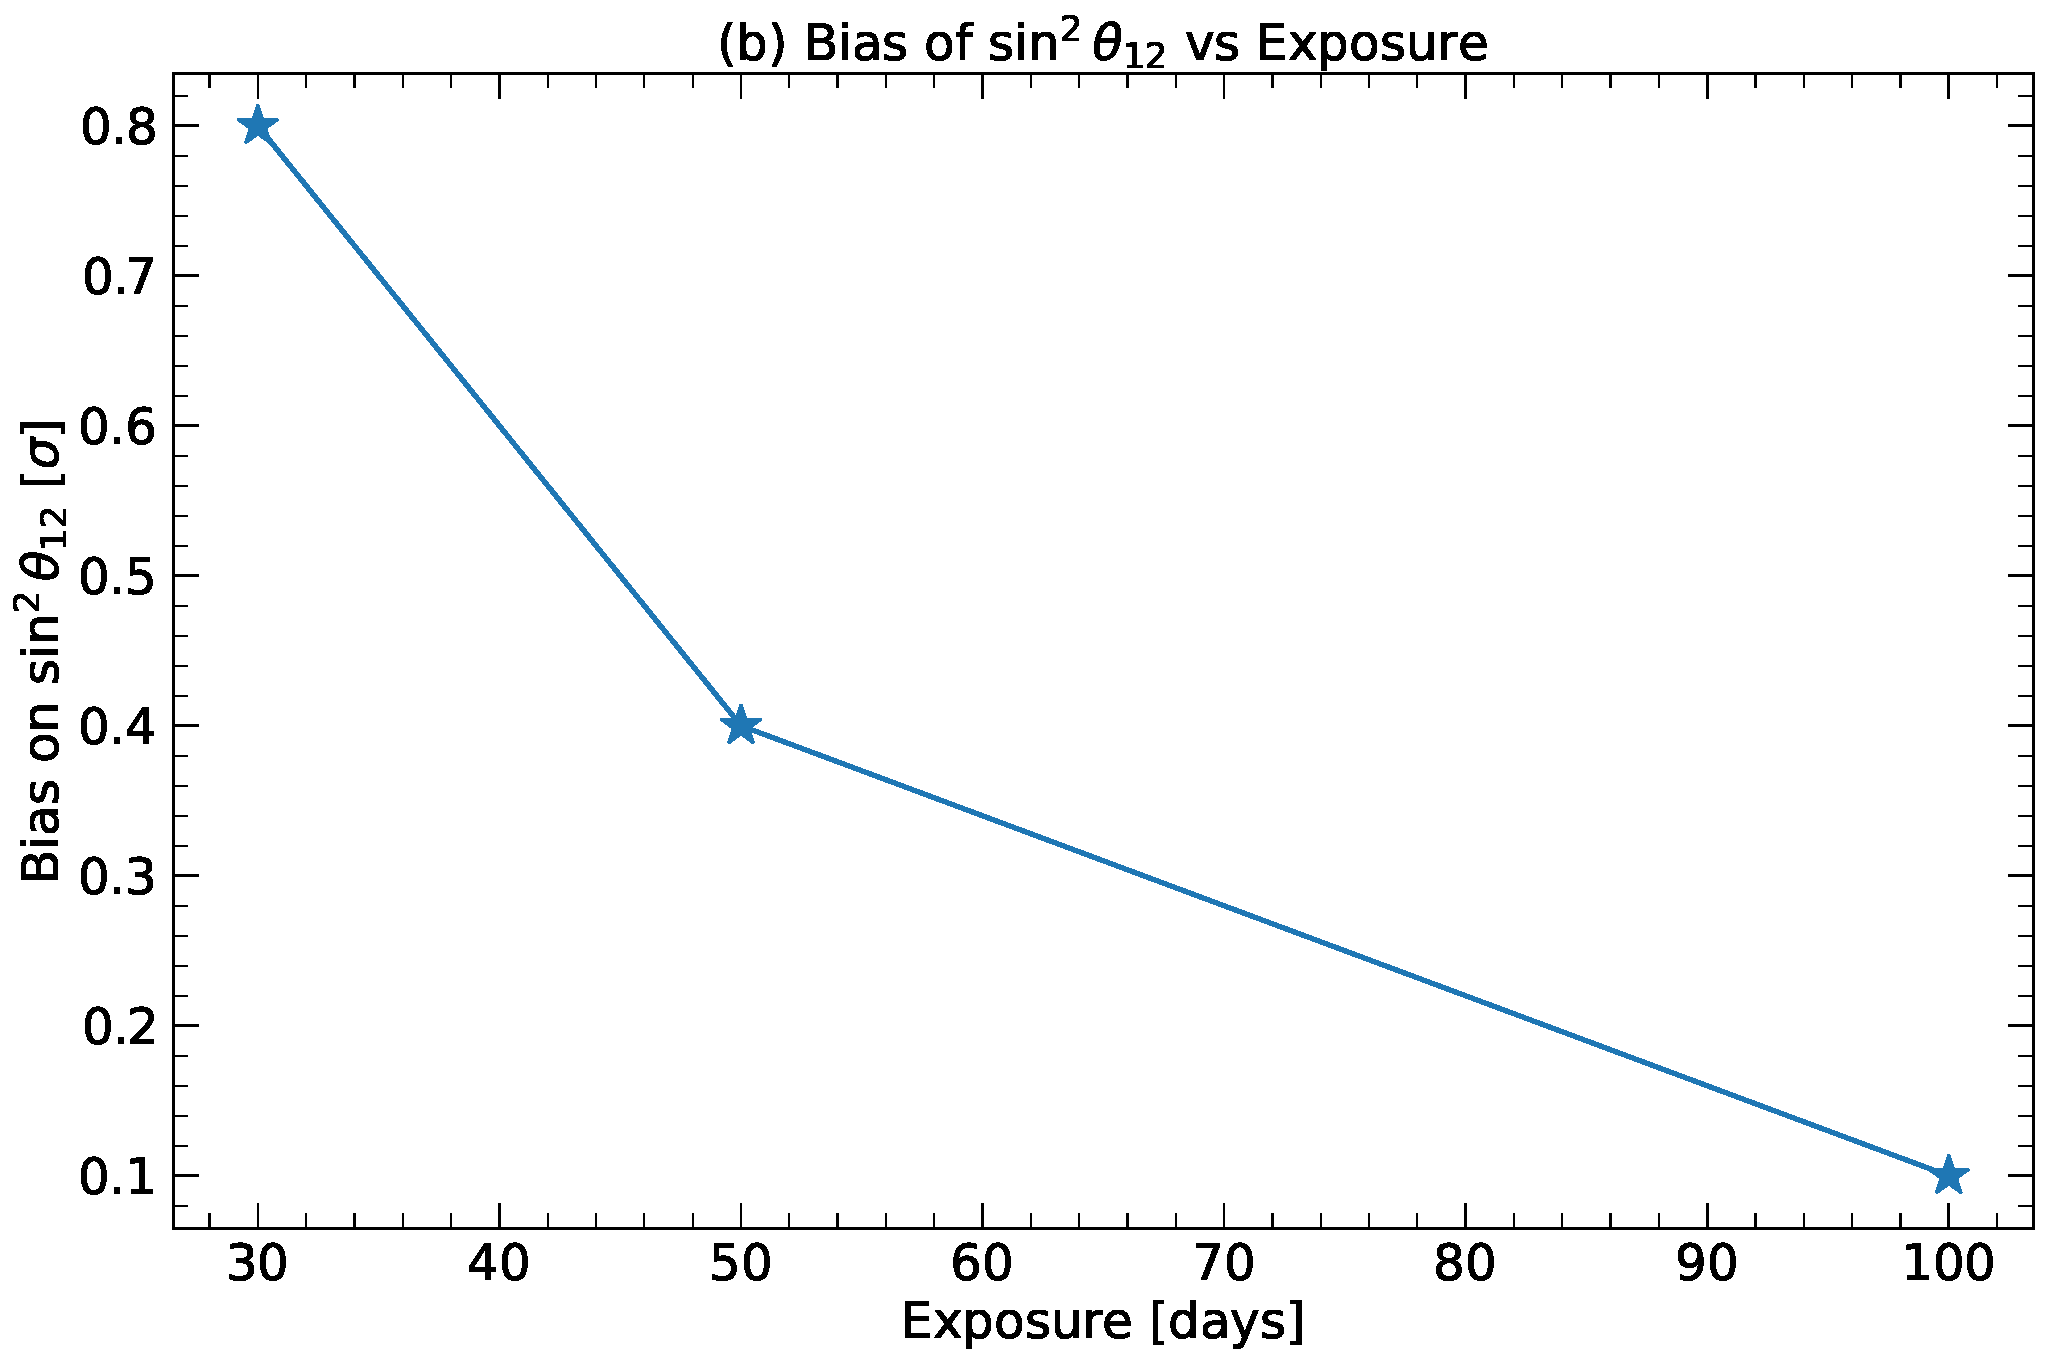
\includegraphics[width=\linewidth]{Img/binning strategy/Bias_of_sin2theta12_vs_exposure.pdf}
      \caption{$\sin^2\theta_{12}$ 偏差随时间的变化.}
      \label{fig:s12_bias}
    \end{subfigure}
    \bicaption{太阳振荡参数偏差随曝光时间的演化。（a）$\Delta m^2_{21}$ 的偏差；（b）$\sin^2\theta_{12}$ 的偏差。}
    {Evolution of the bias of solar oscillation parameters as a function of exposure time. Panel (a) shows the bias of $\Delta m^2_{21}$; panel (b) shows the bias of $\sin^2\theta_{12}$.}
    \label{fig:solar_low_stat_bias}
  \end{figure}
  
图~\ref{fig:solar_low_stat_bias} 给出了两类太阳振荡参数随暴露时间演化的偏差行为：\autoref{fig:dm2_21_bias} 展示了在 30 天、50 天和 100 天曝光条件下 $\Delta m^2_{21}$ 偏差随时间的变化；\autoref{fig:s12_bias} 展示了在 30 天、50 天和 100 天曝光条件下 $\sin^2\theta_{12}$ 偏差随时间的变化。Toy MC 结果与 Asimov 结果进行了比较。蓝色标记表示使用对称 68.27\% 积分法得到的置信区间：即将所有最佳拟合值按升序排列，然后计算分布的第 16 百分位和第 84 百分位。紫色标记与曲线来自对具有相同输入参数的 Asimov 数据集的拟合结果，其最佳拟合值及不确定度由最小化算法给出，并假设服从理想高斯分布。可以看出低统计量下太阳振荡参数存在显著偏差，但随着取数时间增加，偏差明显变小。此外，正如下文所讨论的，采用不同的分 bin 策略可以进一步减小这一效应。


\subsection{偏差与精度的演化}

在低统计数据条件下，谱中的某些 bin 可能只包含极少的事例，甚至没有事例。在这种情况下，χ² 检验统计量会变得不可靠，从而可能在参数估计中引入偏差。减少偏差的一种实际方法是在预期事件数较少的能区，或在整个分析范围内使用更宽的 bin。改变 bin 宽度的影响将在 \autoref{sec:binning_solar} 中进行研究。以下结果均基于名义分 bin，即 20 keV 宽度。

每个参数的偏差定义为最佳拟合值分布的平均值与真实输入值之间的归一化差异：

$$\text{Bias} = \frac{\langle\hat{\theta}\rangle - \theta_{\text{true}}}{\sigma_{\text{68\%}}},$$

其中，$\langle\hat{\theta}\rangle$ 表示5000个伪实验中最佳拟合值的平均值，$\theta_{\text{true}}$ 为名义输入参数值，$\sigma_{68\%}$ 为由上述分布估计得到的不确定度。

\autoref{fig:solar_low_stat_bias} 显示，两种太阳振荡参数在偏差行为上存在差异。对于 $\Delta m^2_{21}$，在所有曝光水平下偏差始终小于 $0.1\sigma$。相比之下，$\sin^2\theta_{12}$ 在 30 天曝光时表现出约 $0.8\sigma$ 的明显偏差，但随着取数时间增加，该偏差显著减小。


需要指出的是，上述结果是在系统误差取名义值的假设下得到的，即假设对系统学参数具有良好的控制。在实际情况下，仅凭 50 天数据难以实现对系统误差（如探测器响应、背景估计等）的如此精确控制。

\subsection{分 bin 策略}\label{sec:binning_solar}

\begin{figure}[h!]
    \centering
    \begin{subfigure}[t]{0.32\textwidth}
      \centering
      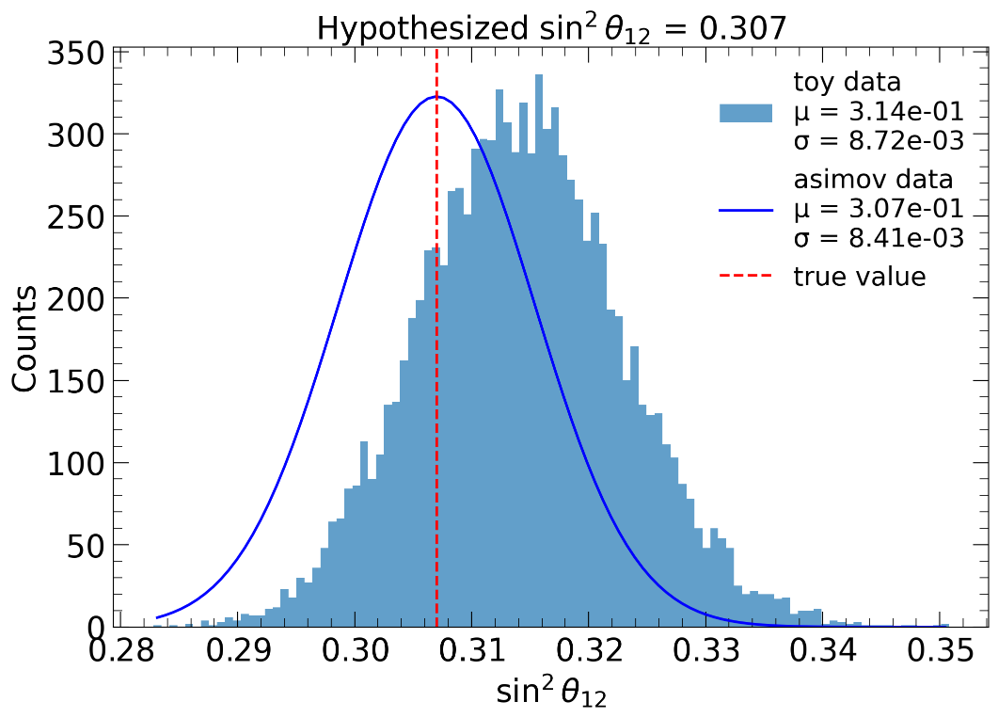
\includegraphics[width=\linewidth]{Img/binning strategy/Jingqin_sinsq12_bias_560bins.png}
      \caption{560 bins.}
      \label{fig:s12_binning_nominal}
    \end{subfigure}
    \hfill
    \begin{subfigure}[t]{0.32\textwidth}
      \centering
      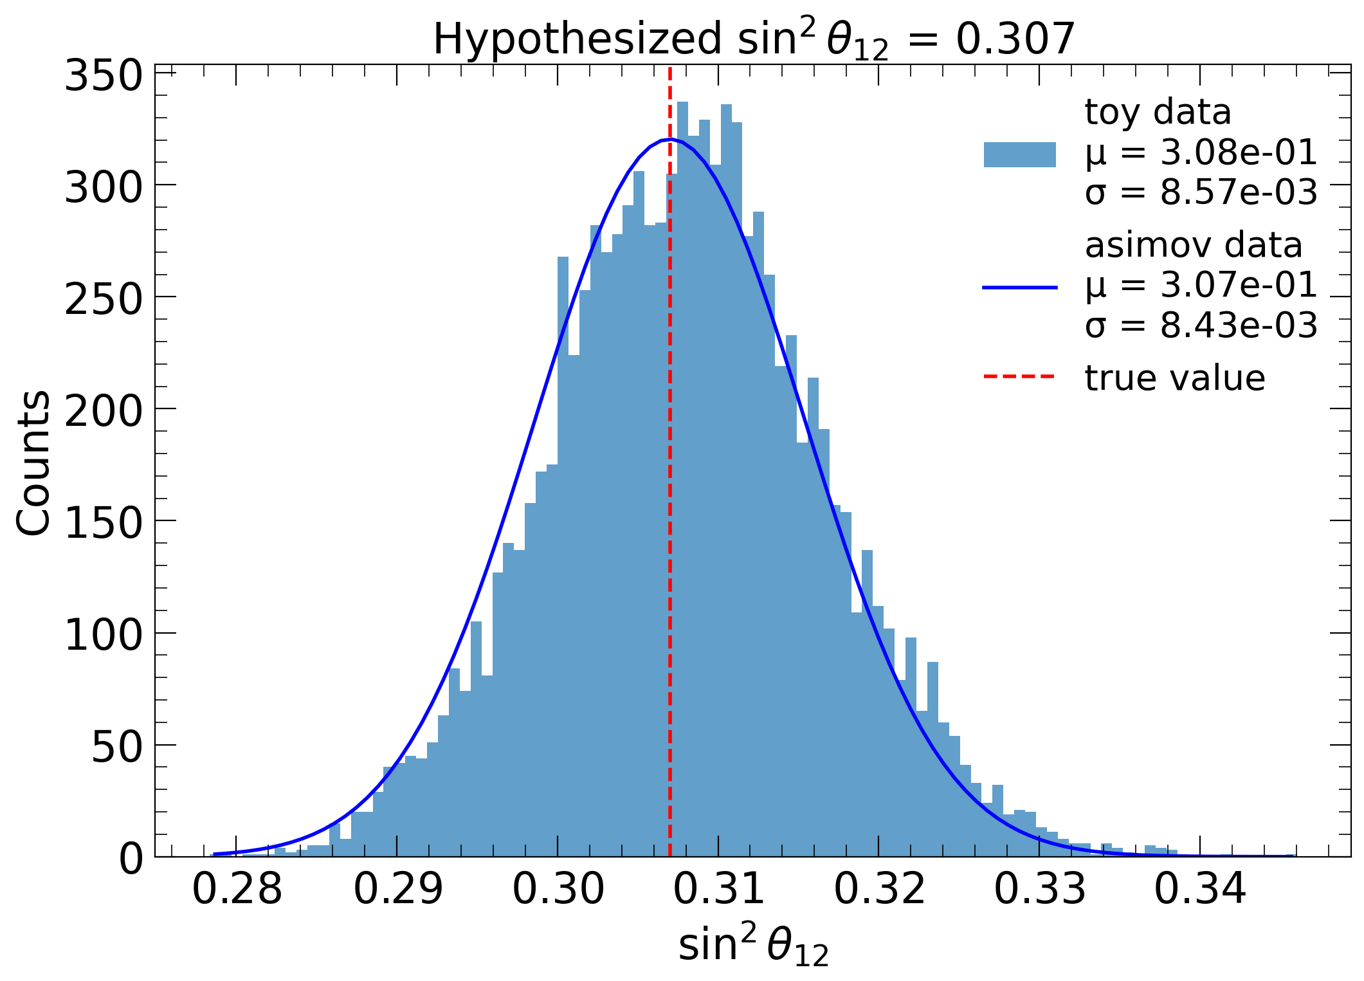
\includegraphics[width=\linewidth]{Img/binning strategy/Jingqin_sinsq12_bias_80bins.png}
      \caption{80 bins.}
      \label{fig:s12_binning_factor7}
    \end{subfigure}
    \hfill
    \begin{subfigure}[t]{0.32\textwidth}
      \centering
      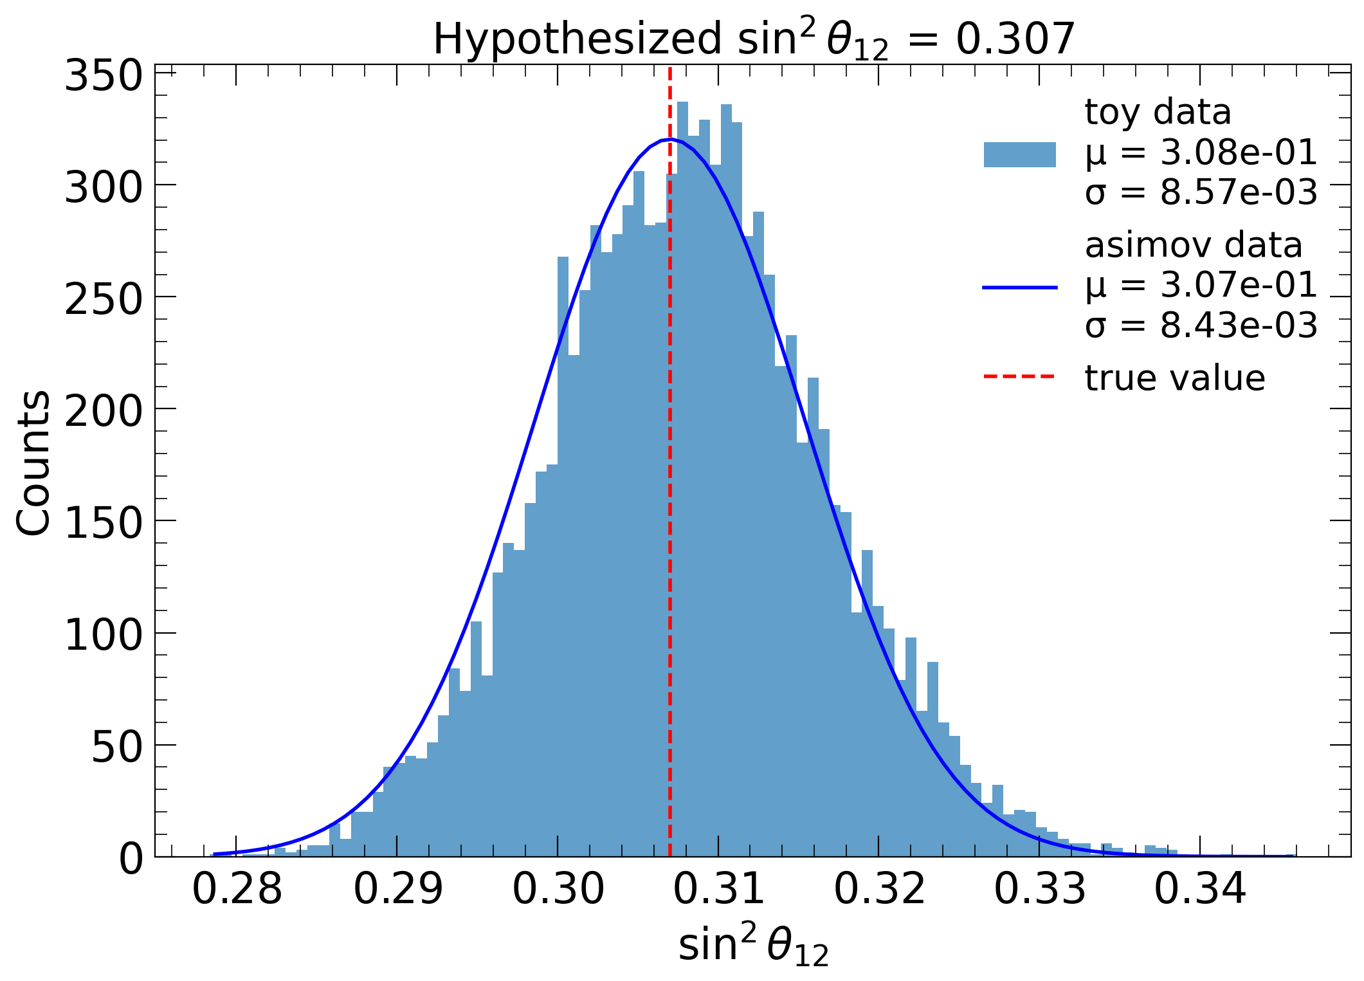
\includegraphics[width=\linewidth]{Img/binning strategy/Jingqin_sinsq12_bias_56bins.png}
      \caption{56 bins.}
      \label{fig:s12_binning_factor10}
    \end{subfigure}
    \bicaption
    {在 30 天曝光条件下，不同重建能谱分 bin 数目下 $\sin^2\theta_{12}$ 最佳拟合值在 10,000 个伪实验中的分布。}
    {Distribution of the best-fit values of $\sin^2\theta_{12}$ from 10,000 pseudo-experiments at 30 days exposure with different numbers of reconstructed energy bins.}
    \label{fig:s12_binning}
  \end{figure}

为研究并减小观测到的偏差，特别是在低曝光（30 天）条件下 $\sin^2\theta_{12}$ 的偏差，开展了一项独立分析。该研究重点考察在 30 天曝光条件下，不同分 bin 配置对偏差的影响。采用 10,000 个伪实验数据集，研究三种不同的分 bin 方案：

\begin{itemize}[leftmargin=*,nosep]
    \item \textbf{560 个 bin}：范围 0.2--12 MeV，与前文名义分 bin 一致；
    \item \textbf{80 个 bin}：范围 0.2--12 MeV，即重分 bin 因子为 7；
    \item \textbf{56 个 bin}：范围 0.2--12 MeV，即重分 bin 因子为 10。
\end{itemize}

\autoref{fig:s12_binning} 展示了在这些不同分 bin 条件下 $\sin^2\theta_{12}$ 最佳拟合值的分布。结果表明，随着 bin 数减少（即 bin 变宽），偏差明显减小。

\begin{figure}[h!]
    \centering
    \begin{subfigure}[t]{0.47\textwidth}
      \centering
      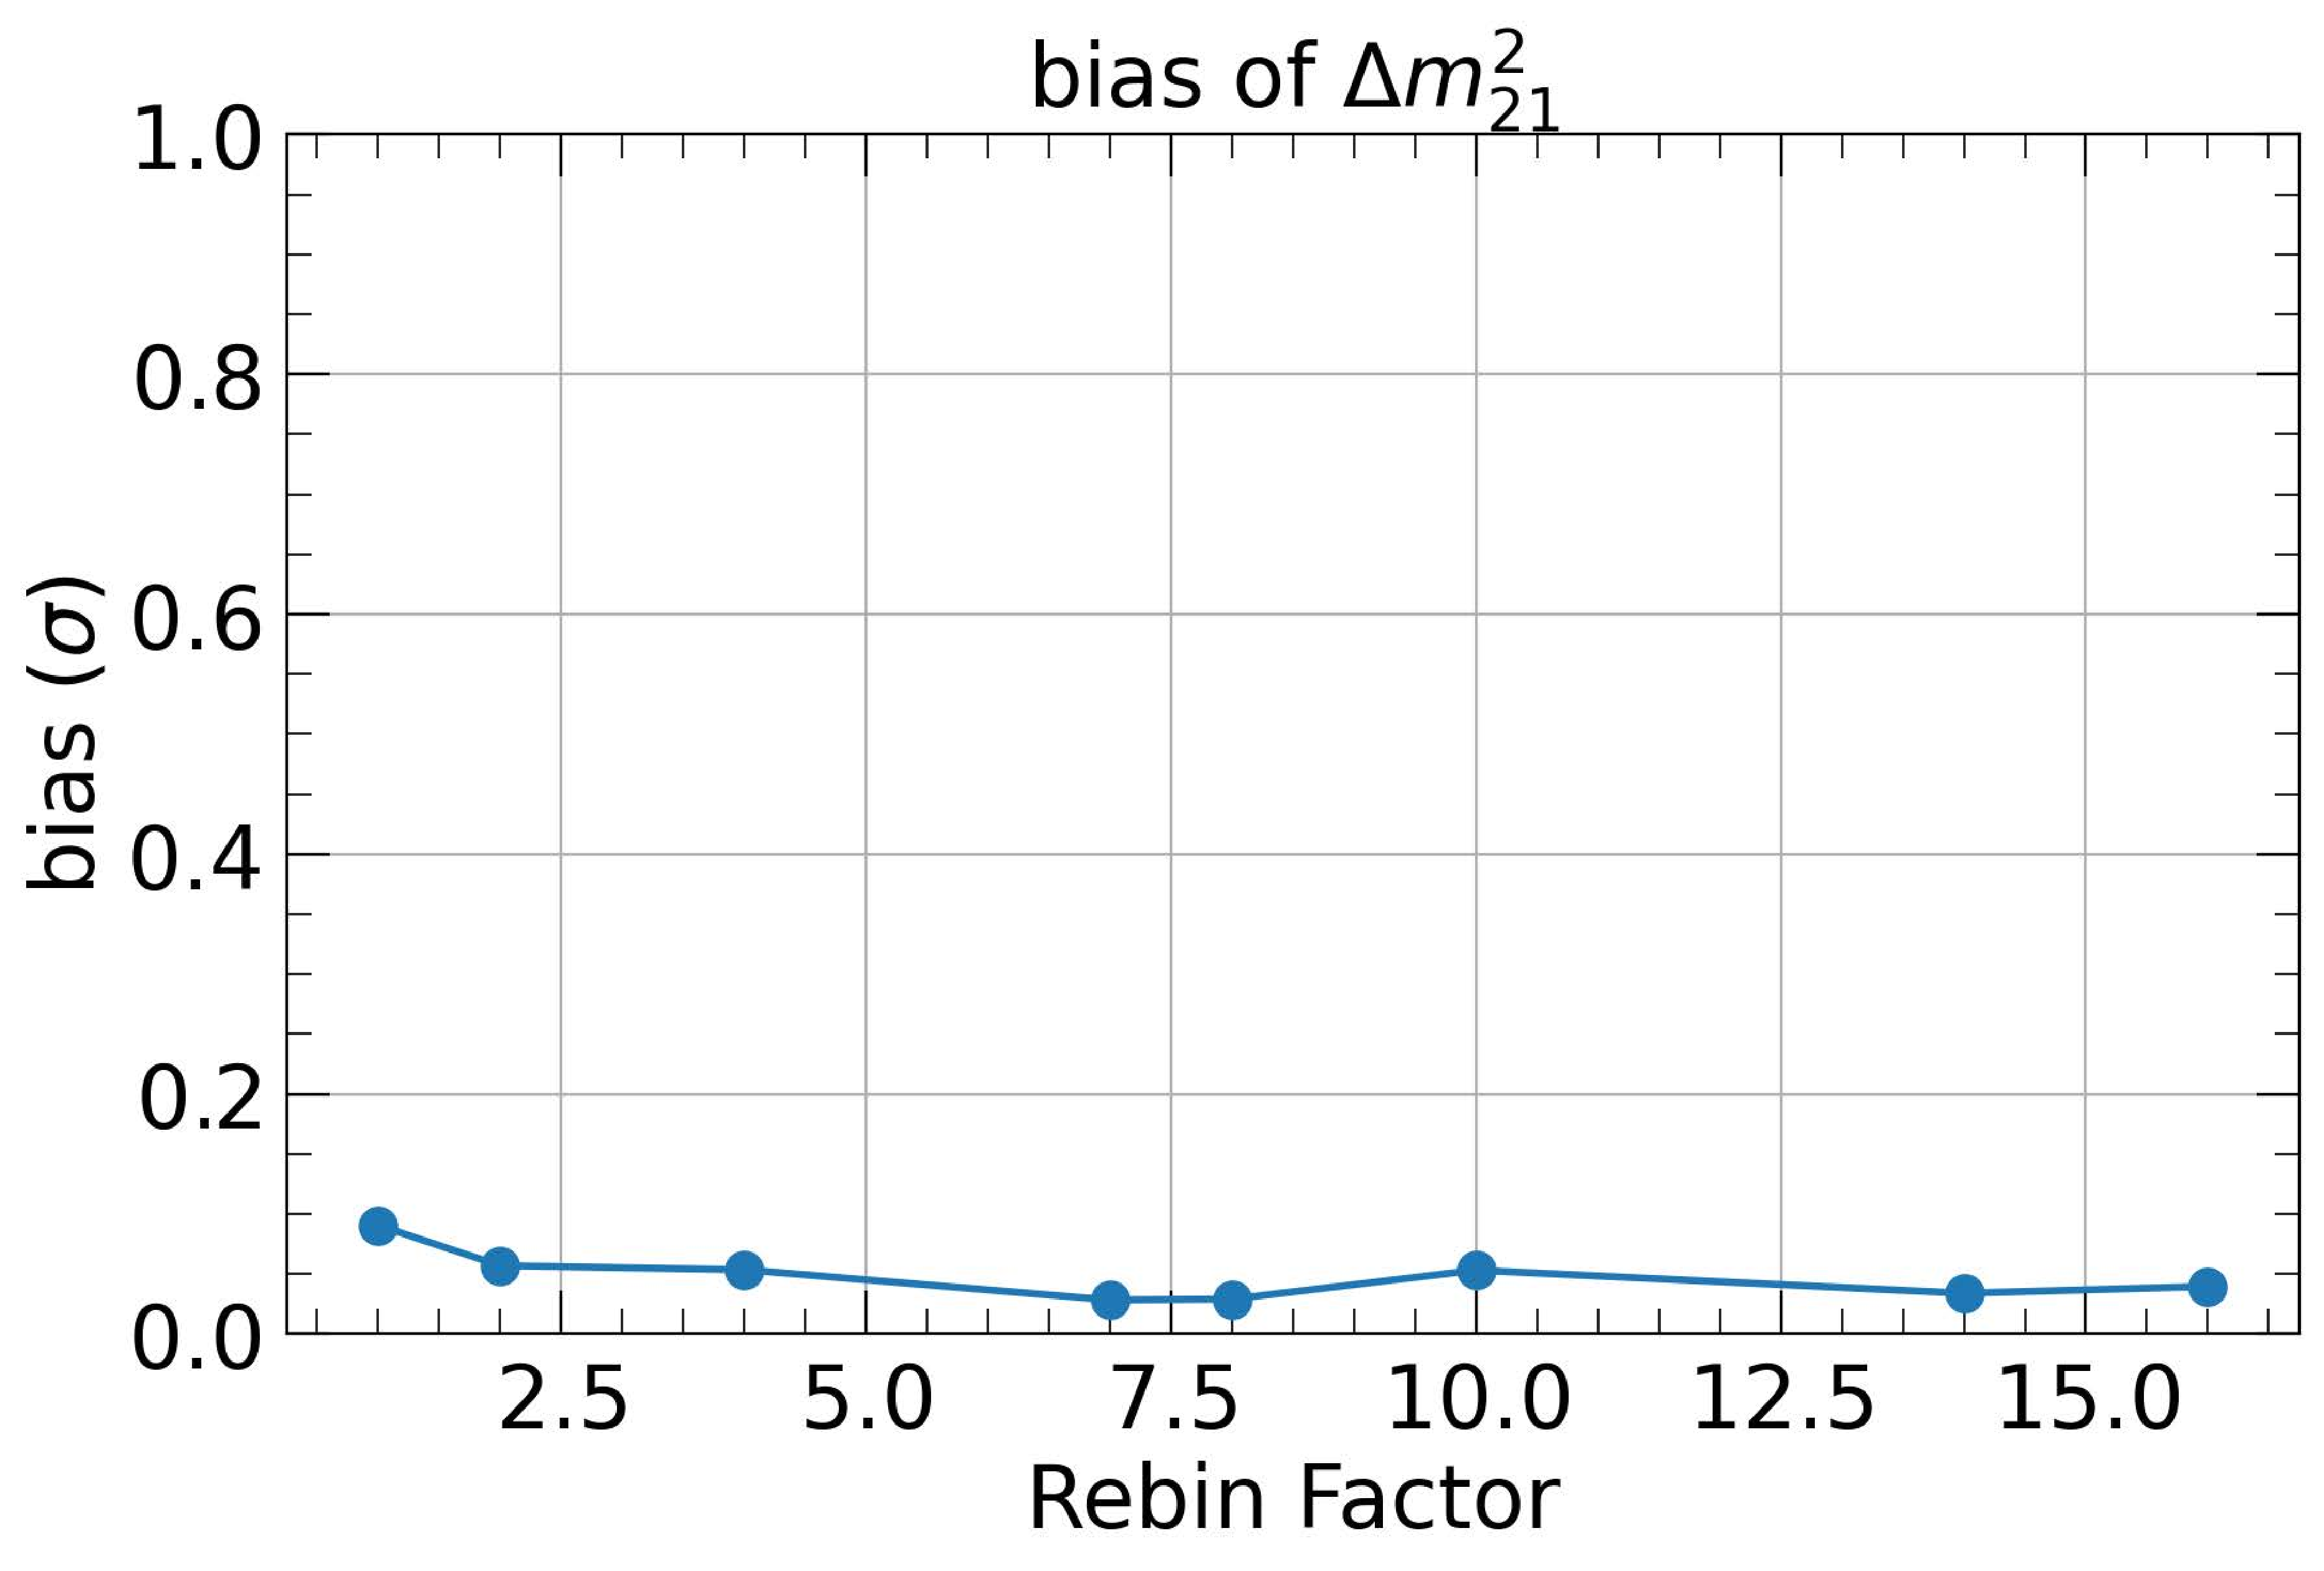
\includegraphics[width=\linewidth]{Img/binning strategy/Jingqin_dmsq21_bias_dif_bins.pdf}
      \caption{$\Delta m^2_{21}$ 偏差随重分 bin 因子的变化。}
      \label{fig:dm2_21_bias_bins}
    \end{subfigure}
    \hfill
    \begin{subfigure}[t]{0.47\textwidth}
      \centering
      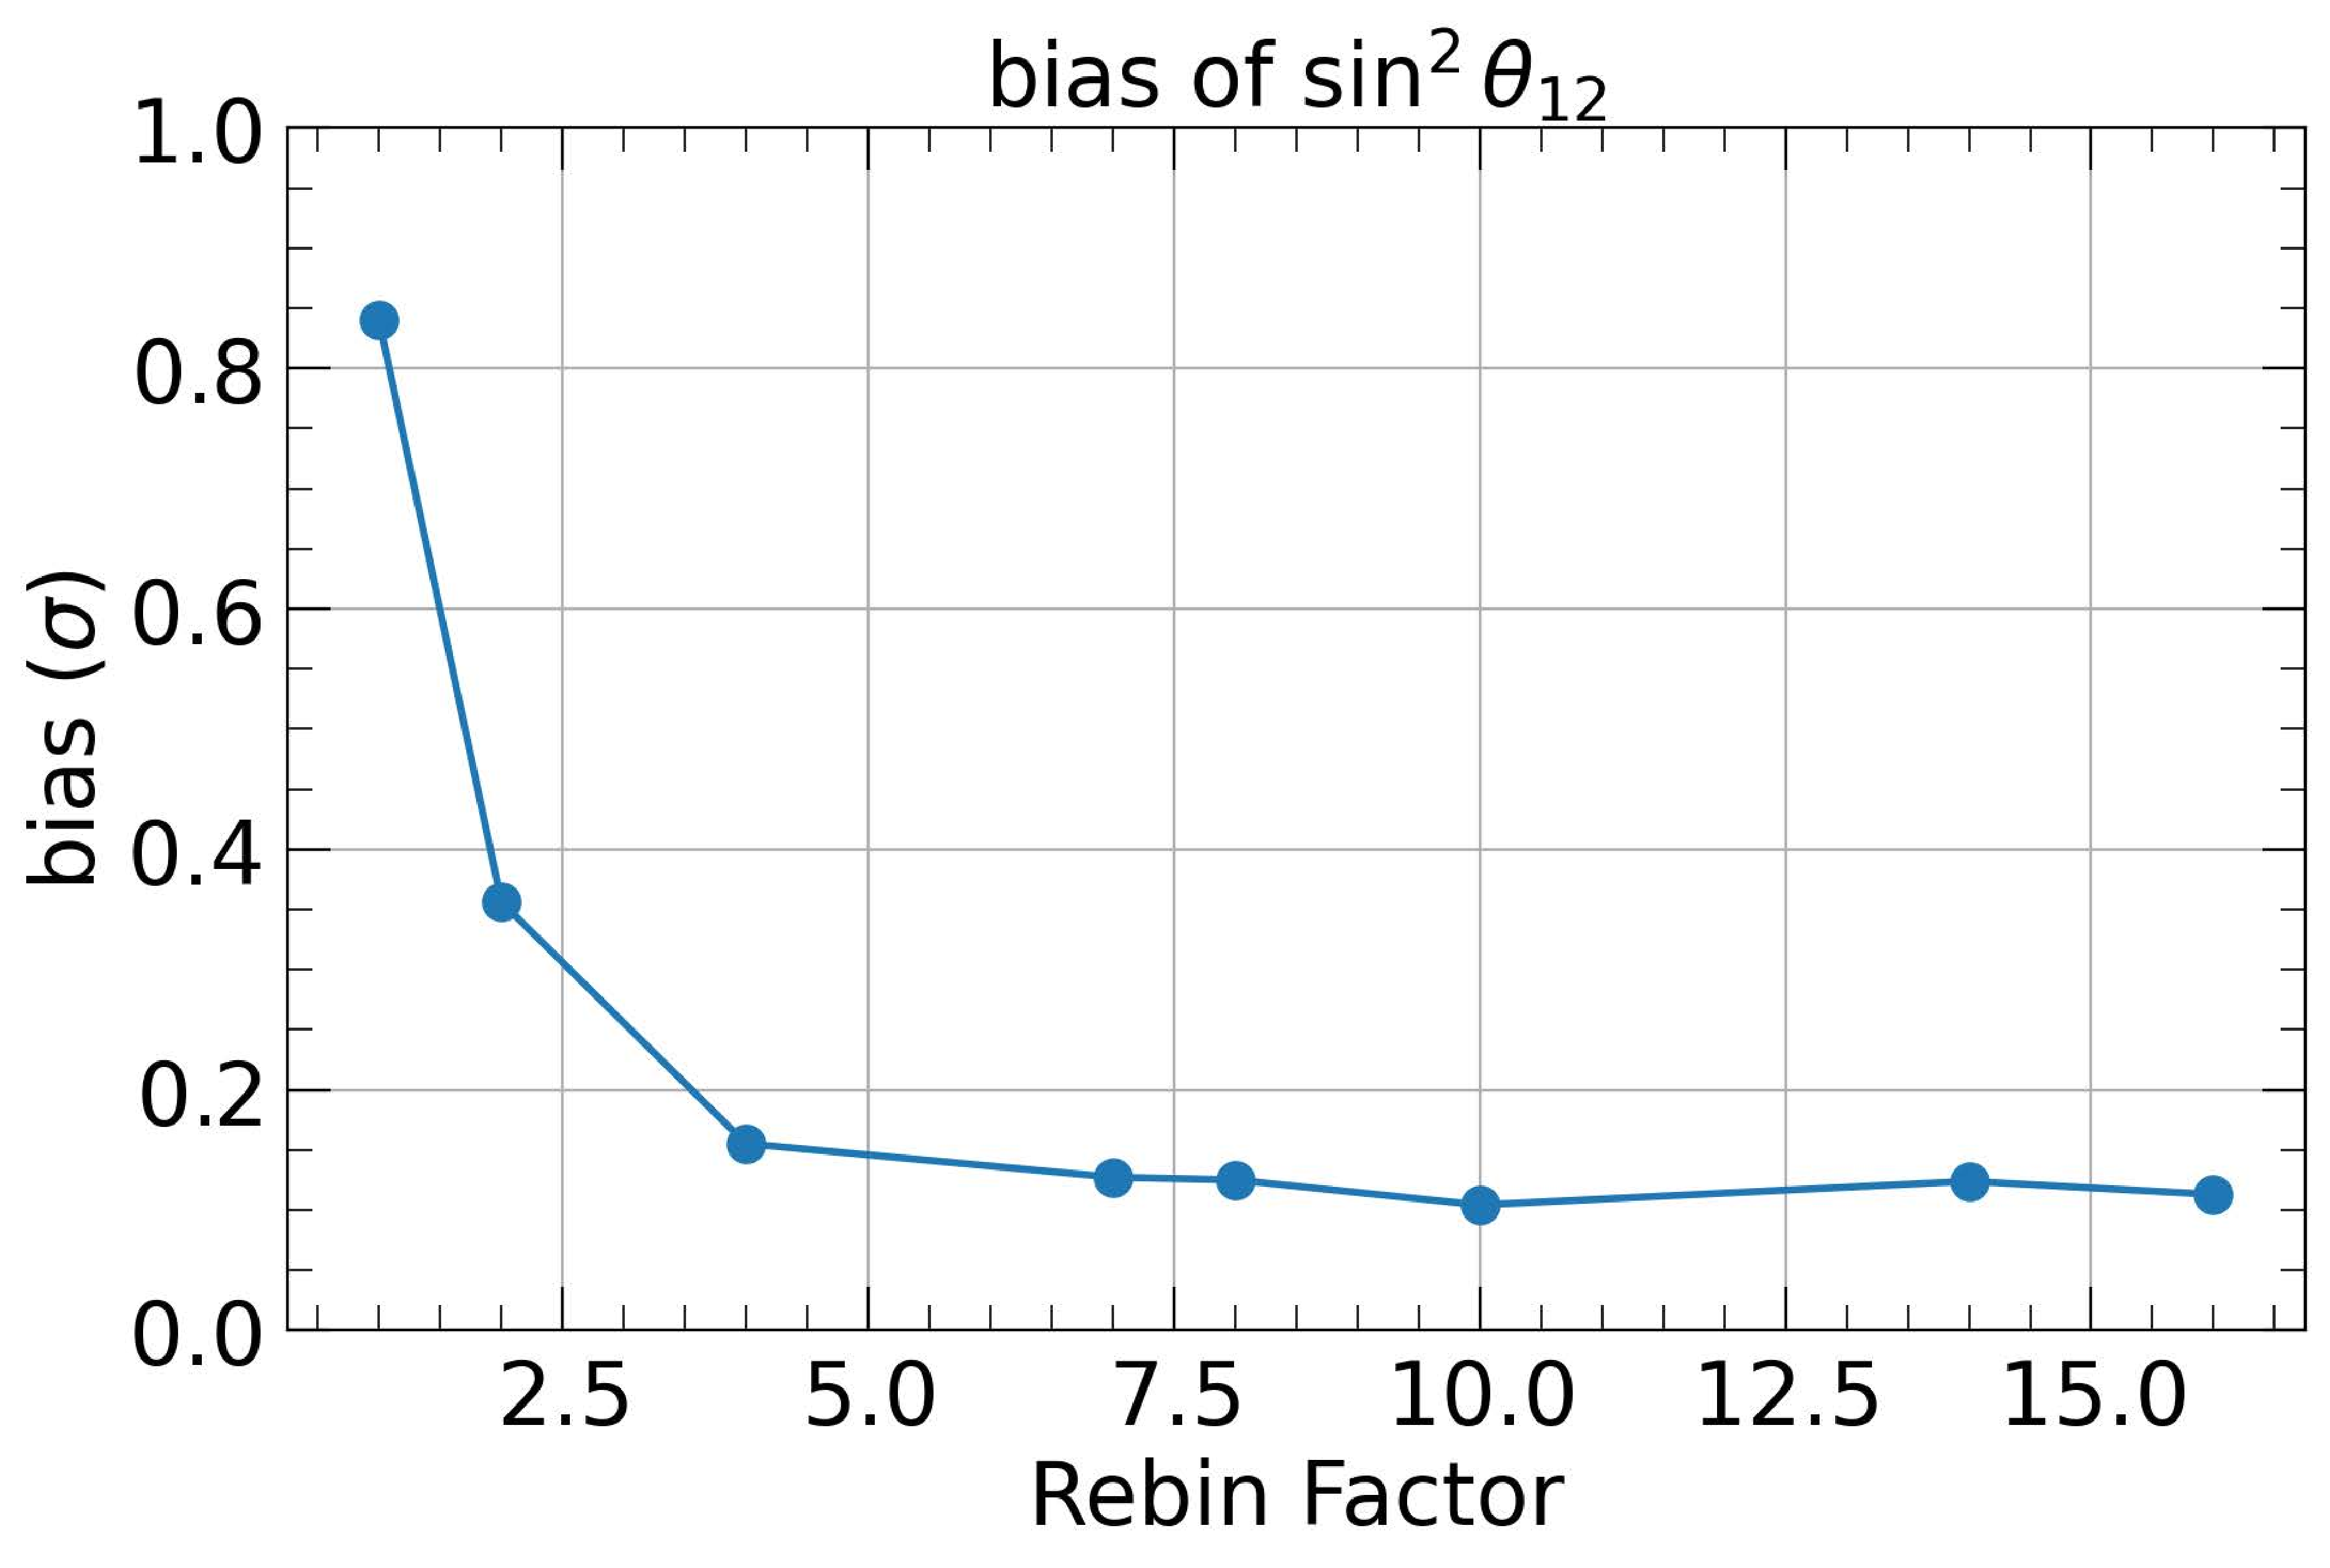
\includegraphics[width=\linewidth]{Img/binning strategy/Jingqin_sinsq12_bias_dif_bins.pdf}
      \caption{$\sin^2\theta_{12}$ 偏差随重分 bin 因子的变化。}
      \label{fig:s12_bias_bins}
    \end{subfigure}
    \bicaption
    {太阳振荡参数偏差随重分 bin 因子的演化。（a）$\Delta m^2_{21}$ 的偏差；（b）$\sin^2\theta_{12}$ 的偏差。}
    {Evolution of the bias of solar oscillation parameters as a function of the rebin factor. Panel (a) shows the bias of $\Delta m^2_{21}$; panel (b) shows the bias of $\sin^2\theta_{12}$.}
    \label{fig:solar_low_stat_bias_bins}
  \end{figure}

\autoref{fig:solar_low_stat_bias_bins} 展示了偏差随重分 bin 因子的变化趋势（以 560 个 bin 为名义配置）。\autoref{fig:dm2_21_bias_bins} 表明，在 30 天曝光下，$\Delta m^2_{21}$ 基本无偏，并且不依赖于重分 bin 因子。另一方面，\autoref{fig:s12_bias_bins} 显示 $\sin^2\theta_{12}$ 对分 bin 策略具有较强依赖性：随着重分 bin 因子增大（bin 数减少），偏差显著下降。从重分 bin 因子 1（560 个 bin，20keV）时约 $0.8\sigma$，降至重分 bin 因子 10（56 个 bin，100keV）时小于 $0.2\sigma$。


\subsection{本节结论}

太阳振荡参数的测量整体上不存在显著挑战。在低曝光条件下，$\Delta m^2_{21}$ 和 $\sin^2\theta_{12}$ 均表现出良好的统计性质。主要结果如下：

\begin{itemize}[leftmargin=*,nosep]
    \item $\Delta m^2_{21}$ 在所有曝光水平下偏差极小（小于 $0.1\sigma$），且不受不同分 bin 选择的影响；
    \item $\sin^2\theta_{12}$ 在极短曝光（30 天）时存在一定偏差，但可通过减少 bin 数（增大 bin 宽至100keV）有效控制；
    \item 在当前研究的名义配置下，JUNO 在首月运行内即可达到优于当前全球结果的测量精度。
\end{itemize}

因此，只要通过适当的探测器刻度和背景建模（尤其是地中微子背景）对系统误差进行良好控制，JUNO 有望在运行最初几个月内实现对太阳振荡参数的世界领先测量。

\section{反应堆中微子能谱分bin策略}

\subsection{早期运行阶段的统计限制与Daya Bay实验约束动机}

在 JUNO 早期运行阶段，反应堆中微子能谱测量面临显著的统计限制。特别是作为近探测器设计的 TAO 子实验，其主要目标是以优异的能量分辨率直接测量反应堆中微子能谱的精细结构。然而在实验启动初期，TAO 尚无法积累足够的统计量以对反应堆谱形进行高精度约束。另一方面，TAO 早期可能无法获得反应堆停堆（reactor-off）数据，这对背景估计的精确性非常重要。这意味着 JUNO 在首篇物理结果中，无法完全依赖自身或 TAO 的数据独立确定反应堆中微子能谱的不确定性。

在缺乏高统计量近点能谱测量的情况下，反应堆中微子模型不确定性将直接传播至远端振荡分析中。由于 JUNO 采用前向折叠（forward-folded）能谱拟合方法，理论反应堆能谱需要经过振荡效应、IBD 截面以及探测器响应函数卷积后，与重建能谱进行比较。因此，输入反应堆能谱的形状误差会以高度相关的方式影响最终振荡参数的提取。如果不加控制，这种模型依赖可能在统计误差尚未完全主导时，就成为系统误差的主要来源。

而Daya Bay 实验已积累了超过 550 万个电子反微中子事件的高统计数据。这些高统计数据可为 JUNO 提供对初始反应堆反中微子能谱的有力约束，从而显著降低远场振荡分析中由谱形不确定性引入的系统误差。

基于上述考虑，JUNO 首篇物理结果计划采用与大亚湾实验（Daya Bay, DYB）的联合分析策略。大亚湾近探测器具有极高统计量的反应堆中微子能谱测量结果，可为反应堆谱形提供外部约束。然而，由于 DYB 探测器能量分辨率相对有限，其对谱形精细结构的约束能力存在固有尺度限制。因此，在将 DYB 数据引入联合拟合框架时，必须对反应堆能谱的自由度进行合理分段，使其既能有效吸收模型不确定性，又不超出 DYB 实验的约束能力。

这一本质上的统计与系统误差之间的张力，构成了反应堆能谱分段（segmentation）策略设计的出发点。下一节将介绍联合分析框架及其数学形式化描述。

\subsection{联合分析框架}

为了在联合拟合中把近场高统计信息形式化地纳入，我们采用对大亚湾数据的 χ² 约束。具体地，我们将大亚湾测得的 prompt 能谱 $\boldsymbol{M}^{\rm DYB}$（经归一化并去除振荡与乏燃料/非平衡修正）与模型预测 $\boldsymbol{T}^{\rm DYB}$ 进行比较，得到如式~(\ref{eq:Chisq:DYB}) 所示的 $\chi^2_{\mathrm{DYB}}$。其中协方差矩阵 $\mathbf{Cov}$ 包含了统计不确定度以及探测、背景和反应堆相关的系统误差分量，模型预测 $\boldsymbol{T}^{\rm DYB}$ 在构造时包含 IBD 截面、液体闪烁体非线性、能量分辨以及 IAV 等探测器效应（均按文献~\cite{PhysRevLett.134.201802} 的响应模型处理）。在联合最小化时，我们将 JUNO 的 χ² 与上述 $\chi^2_{\mathrm{DYB}}$ 相加，再加上来自大亚湾对 $\sin^2\theta_{13}$ 与 $\Delta m^2_{31}$ 的外部高精度先验项，得到总目标函数式~(\ref{eq:Chisq:Total})。

（注：式~(\ref{eq:Chisq:Total}) 中的 $\chi^2_{\rm JUNO}$ 包含 JUNO 观测谱、背景项、探测器响应与其它拉项约束；在实现时我们按段级参数 $\{\alpha_i\}$ 将 DYB 的约束映射到 JUNO 的谱预测中。）

为了利用近点探测器对反应堆能谱的约束，我们将 Daya Bay实验提供的经过去振荡、去 SNF/Non-Eq 修正并按每次裂变归一化的提示能谱 $\boldsymbol{M}^{\rm DYB}$ 纳入联合拟合。Daya Bay 的数据项采用带完整协方差矩阵的 χ²：  
\begin{equation}  
\chi^2_{\rm DYB} = (\boldsymbol{M}^{\rm DYB} - \boldsymbol{T}^{\rm DYB})^\top \mathbf{Cov}^{-1} (\boldsymbol{M}^{\rm DYB} - \boldsymbol{T}^{\rm DYB}),  
\label{eq:Chisq:DYB}  
\end{equation}  
其中 $\boldsymbol{T}^{\rm DYB}$ 为我们用相同反应堆谱模型和 DYB 给定的响应映射（包括 IBD 截面、非线性、分辨率与 IAV 等效应）计算得到的预测谱，$\mathbf{Cov}$ 为 DYB 提供的完整协方差矩阵（包含统计与各类系统误差）。将 DYB 纳入能显著约束反应堆谱的系统不确定性并降低模型相关偏差。

此外，我们还在拟合中引入来自 Daya Bay 等实验对 $\sin^2\theta_{13}$ 与 $\Delta m^2_{31}$ 的外部约束（Gaussian prior），作为额外的拉项。最终的总目标函数为  
\begin{equation}
\begin{aligned}
\chi^2_{\rm Total}
&= \chi^2_{\rm JUNO} + \chi^2_{\rm DYB} \\
&\quad + \left( \frac{\sin^2\theta_{13} - \sin^2\theta_{13}^{\rm DYB}}{\sigma(\sin^2\theta_{13}^{\rm DYB})} \right)^2 \\
&\quad + \left( \frac{\Delta m_{31}^2 - \Delta m_{31}^{2,\rm DYB}}{\sigma(\Delta m_{31}^{2,\rm DYB})} \right)^2 \, .
\end{aligned}
\label{eq:Chisq:Total}
\end{equation}

为降低反应堆谱形不确定性对远场振荡分析的影响，我们采用将 Daya Bay 的高统计近点能谱数据引入 JUNO 拟合的联合分析框架。联合分析的关键思路是对连续的反应堆 $\bar\nu_e$ 能谱进行分段（energy segmentation），并用近点的高统计数据对每一段的归一化自由度施加外部约束，从而在保证灵敏度的同时控制模型依赖性。


具体做法如下：

\begin{enumerate}
  \item \textbf{谱段化（segmentation）}
  
  将初始反应堆能谱 $S(E)$ 在能量空间上划分为若干不重叠的能段 $\{I_i\}$，并把原始连续谱表示为各段基形 $S_i(E)$ 的线性组合：
  $$
    S(E)\;\approx\;\sum_{i}\alpha_i\,S_i(E),\qquad S_i(E)\equiv S(E)\,\mathbf{1}_{E\in I_i},
  $$
  其中 $\alpha_i$ 为第 $i$ 段的归一化因子（拟合参数），$\mathbf{1}_{E\in I_i}$ 为段指示函数。
  
  \item \textbf{段内保持谱形固定、段间自由调节}
  
  在每一能段 $I_i$ 内假定谱形（相对能量依赖）由基底 $S_i(E)$ 给出且保持不变，仅通过整体缩放因子 $\alpha_i$ 来调节该段的强度。不同段之间的相对强度由 $\{\alpha_i\}$ 在拟合过程中独立调整，从而将连续谱的无限维自由度离散化为一组有限维参数问题。
  
\item \textbf{近点数据的外部约束}
  
  作为近点高统计量数据的代表实验，Daya Bay 数据对这些段级归一化因子给予外部约束：在联合拟合中加入一项表征 DYB 与模型偏差的 χ²（或协方差先验），使得 $\{\alpha_i\}$ 在拟合时既能响应远场（JUNO）数据的需求，又受近点高统计数据的牵引与正则化。数学上，联合目标可写为式~(\ref{eq:Chisq:Total})，其中 $\theta$ 表示振荡参数，$\chi^2_{\rm DYB}$ 给出 $\{\alpha_i\}$ 的先验信息或协方差约束（其具体形式见式~(\ref{eq:Chisq:DYB})）。
\end{enumerate}


将连续谱自由度离散化为段间归一化因子，可以显著降低谱形不确定性对振荡参数估计的敏感性；通过引入近点高统计约束，联合拟合能够抑制模型引起的偏差，同时保留远场对振荡结构（例如 $L/E$ 谱振荡）的辨识能力；段宽（segment size）为关键自由量：若段宽过小，会超出近点探测器（DYB）在能量分辨与统计上的约束能力，导致拟合出现非物理波动或过拟合；若段宽过大，则反应堆模型依赖性增强，无法反映局部谱形差异。故段宽的选择必须在“模型相关系统误差”与“统计不确定性／约束能力”之间取得平衡。
        
综上所述，本节采用的分段联合拟合策略实质上是用 Daya Bay 的高统计近点信息“锚定”反应堆谱的局部形状（local shape），从而为 JUNO 的远场振荡分析提供稳健且可控的谱形先验。后续小节将给出具体的段划方案、Toy-MC 验证设计与最终的段宽选择依据。
    
\subsection{半模型独立方法}

反应堆能谱是占主导地位的系统误差来源。我们采用一种半模型独立的策略：利用Daya Bay 的高统计数据约束基准谱形，而理论上的 Huber–Müller（HM）预测仅用于 JUNO 特有的修正项（例如不同堆芯间的裂变份额差异、乏核燃料与非平衡校正等）。
为在尽量减少理论模型依赖的前提下，充分利用近点高统计数据对反应堆谱形的约束，我们采用一种半模型独立（semi-model-independent）的谱预测与拟合框架。对第 $r$ 号反应堆，入射中微子谱记为

\begin{equation}\begin{aligned}
\phi'_r(E_\nu)
&=T_{\rm live}\,
\frac{P_r}{\sum_{r,i} f_{r,i}\,\varepsilon_{r,i}}
\Bigg[
S_{\rm model}(E_\nu)
+\sum_i f_{r,i}\,S_i^{\rm HM}(E_\nu)
\Bigg] \\
&\quad
+ T_{\rm live}\,\phi^{\rm SNF}_r(E_\nu)
+ T_{\rm live}\,\phi^{\rm NonEq}_r(E_\nu)
+ \sum_i \Delta f_{r,i}\,S_i^{\rm HM\text{-}Bump}(E_\nu)\, .
\end{aligned}
\label{eq:phi:semi-model-independent}
\end{equation}

下面逐项解释该表达式的物理意义、实现方法与半模型独立实现细节。

\paragraph*{（1）归一化因子与探测器活跃时间}
前置因子 $T_{\rm live}\frac{P_r}{\sum_{r,i} f_{r,i}\,\varepsilon_{r,i}}$ 为总体归一化／标度项：$P_r$ 为第 $r$ 号堆的热功率，$\varepsilon_{r,i}$ 为探测器对应同位素 $i$ 的裂变能量，$T_{\rm live}$ 为活跃取数时间。该部分仅决定总事件率尺度，与谱形的“局部形状”是分离的，便于在拟合中将幅值与形状分别处理。

\paragraph*{（2）模型无关的主项 $S_{\rm model}(E_\nu)$}
$S_{\rm model}$ 表示一套“通用基底”或主谱形模板，既可以取名义的 Huber--Müller（HM）模型、summation 模型，也可以用“经验段化（segment）基底”直接构造。在半模型独立（semi-model-independent）框架中，关键点不是把 $S_{\rm model}$ 当作“绝对真实值”，而是将其作为起始形状／段内模板：通常把能量区间划分为若干段（segments），段内的相对谱形由 $S_{\rm model}$ 给出（即段内刚性），但每段的整体归一化作为自由参数（或带 DYB 先验的 nuisance）在拟合中允许独立浮动，即“段内刚性、段间自由”，从而实现对模型的弱依赖而非完全倚赖。

\paragraph*{（3）非平衡修正项 $\phi^{\rm NonEq}_r(E_\nu)$}
对应项为 $T_{\rm live}\,\phi^{\rm NonEq}_r(E_\nu)$。该项表示由于长寿命裂变产物尚未达到稳态所引起的非平衡修正。在本分析中，该贡献被整体作为一个小的能量相关通量修正项处理，而不再在同位素层面展开，其不确定度通过独立协方差矩阵传播。

\paragraph*{（4）乏燃料贡献 $\phi^{\rm SNF}_r(E_\nu)$}
对应项为 $T_{\rm live}\,\phi^{\rm SNF}_r(E_\nu)$。该项表示堆外乏燃料池中残余 $\beta$ 衰变所产生的反中微子贡献。由于其强度相对主反应堆裂变通量较小，且谱形可通过堆厂运行记录估算，因此作为一个独立的附加通量项处理。

\paragraph*{（5）补偿／差分项 $\sum_i \Delta f_{r,i}\,S_i^{\rm HM\text{-}Bump}$（关键项）}
令 $\Delta f_{r,i}\equiv f_{r,i}^{\rm JUNO}-f_i^{\rm DYB}$ 表示 JUNO（或某个堆）与 DYB 参考之间的裂变份额差异。补偿项把同位素级别的“已知／观测到的大尺度谱形偏差”（例如 HM-bump）作为基函数 $S_i^{\rm HM\text{-}Bump}$ 投影，并用 $\Delta f_{r,i}$ 线性组合来修正。该设计的物理动机是：当利用 DYB 的高统计谱去“锚定”整体谱形时，JUNO 与 DYB 在燃料构成上不可避免有差别，差别会引起可预测的谱形偏移；把这部分显式写成线性补偿项，使得联合拟合时 DYB 所能很好约束的“共同成分”与 JUNO 特有的“堆芯差分成分”被明确区分，从而减少把堆芯差异误认作振荡信号的风险。

从式~(\ref{eq:phi:semi-model-independent})的分解可以直接看出分段选择为何会引发上述的二择一问题。式中共有几类贡献：

\begin{itemize}
\item 一个由 $S_{\rm model}(E_\nu)$ 与若干反应堆中微子能谱基底（segments）所表示的“主项”，它提供了段内相对谱形的模板与段间的归一化自由度，其中段内谱形是刚性的，依赖于模型；
\item 一组同位素／模型相关的结构项（如使用 HM-Bump 模型的差分投影
  $\sum_i \Delta f_{r,i}\,S_i^{\rm HM\text{-}Bump}$），这一部分是模型相关的；
\item 若干次要的整体通量修正项（$\phi^{\rm NonEq}$、$\phi^{\rm SNF}$ 等），这部分也部分依赖于模型。
\end{itemize}
    

因此，分段策略等价于在模型空间中引入了一组附加自由度（段系数），这些自由度用于在拟合中调整 $S_{\rm model}$ 的局部归一化以匹配数据。问题的关键在于：数据（主要由 Daya-Bay 等近点实验提供的约束）对这些自由度的约束能力是有限的。若我们把能量区间分成 $N_{\rm seg}$ 段，则会新增约 $N_{\rm seg}$ 个段系数自由度；这些自由度必须由近点数据通过协方差或 likelihood 条款来约束，否则拟合会出现不受控的局部波动，从而导致模型依赖性增强，系统误差增大。因此核心矛盾是系统误差与统计误差的平衡。

\paragraph*{核心矛盾（物理与统计的折中）}
在采用“段化（segment）”策略用近点高统计数据约束反应堆谱时存在根本性的二择一：

\begin{itemize}
\item \textbf{分段过多（段宽太细）}
\begin{itemize}
\item \textbf{问题：}当段宽小于近点探测器（如 Daya Bay）的有效能量分辨尺度时，近点数据无法对每一段提供独立而可靠的约束，统计误差增大；拟合会出现未被约束的高频自由度，导致在重建谱中呈现振荡型或非物理性的结构（over-fitting / unphysical wiggles）。
\item \textbf{后果：}拟合过程可能用段系数“吸收”真实的振荡微结构（例如由 $\Delta m^2_{31}$ 引起的小尺度波动），从而弱化对振荡参数的灵敏度或引入偏差。
\end{itemize}
\item \textbf{分段过少（段宽太宽）}
\begin{itemize}
\item \textbf{问题：}段间自由度被过度限制，段内谱形假定刚性——若真实谱存在局部结构或堆芯间差异，这些将无法被段化自由度吸纳，只能依赖理论模型来修正。
\item \textbf{后果：}对理论谱模型的依赖增强，模型相关系统误差（model-dependent bias）被放大，使振荡参数测量的系统容差变差且难以量化。
\end{itemize}
\end{itemize}

因此，段宽选择本质上是在“模型相关系统误差”和“统计不确定性／约束能力”之间寻找平衡。

\subsection{Toy-MC 研究}

为量化上述折中并给出可操作的分段（段宽）选择准则，我们设计一组 Toy-MC 实验，用相同的拟合框架进行拟合，比较两种代表性情况下振荡参数的精度：

\begin{itemize}
\item \textbf{固定反应堆模型情形（Fixed model）：}使用单一名义谱（例如 Huber--Müller 模型或 summation 模型）生成伪数据。该情形评估统计波动与方法本身的行为。
\item \textbf{变化反应堆模型情形（Model-variation）：}基于最新的核数据库构建一组带有精细结构的反应堆能谱，在生成伪数据时对反应堆谱引入物理上合理的扰动（例如随机化的分支比和同位素产额），然后使用名义模板拟合。该情形评估“模型依赖”对振荡参数的影响。
\end{itemize}

\textbf{目标：}对一系列候选段宽（segment widths）比较两类情形下对关键振荡参数的精度（precision），并据此挑选使模型依赖引入的额外系统误差最小的段宽。

\paragraph*{Toy-MC 实验设计}
反应堆中微子能谱范围为 $1.8$--$13\,\mathrm{MeV}$，在该能区范围内选取不同的分 bin 策略。对于每个分段策略，生成 5000 个伪实验数据集。

\begin{figure}[htbp]
\centering
\begin{subfigure}[t]{0.45\textwidth}
\centering
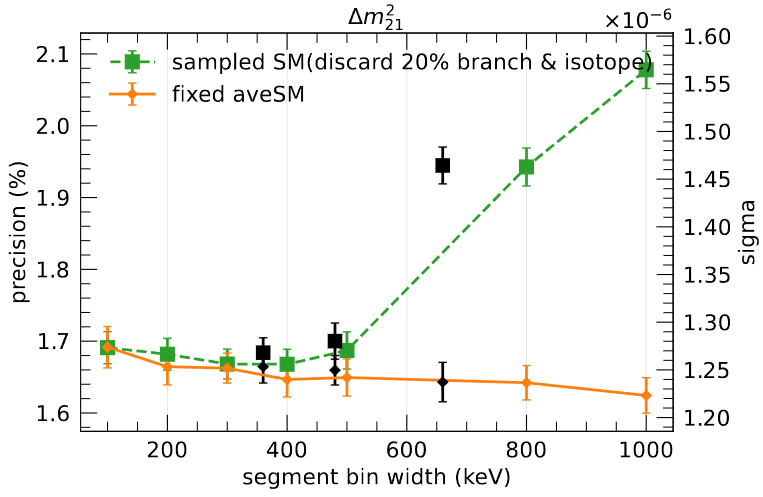
\includegraphics[width=\linewidth]{../groupA_technote/5_oscillation/segment_dmsq21.png}
\caption{}
\label{fig:segment_dmsq21}
\end{subfigure}
\hfill
\begin{subfigure}[t]{0.45\textwidth}
\centering
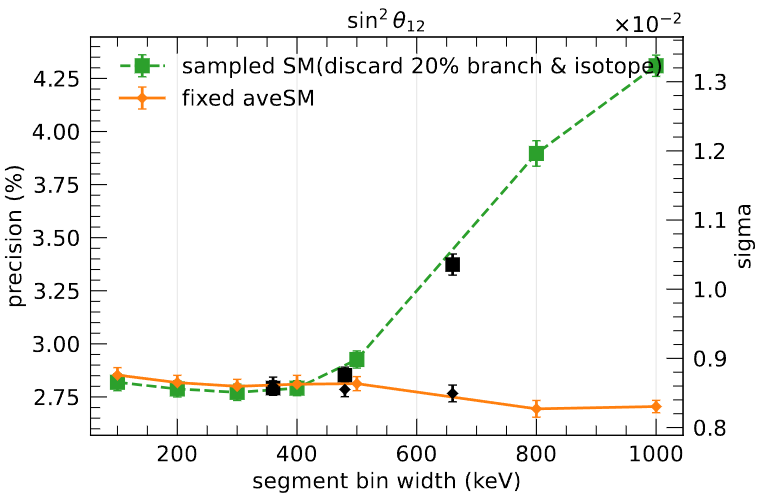
\includegraphics[width=\linewidth]{../groupA_technote/5_oscillation/segment_sinsq12.png}
\caption{}
\label{fig:segment_sinsq12}
\end{subfigure}
\bicaption[段宽对振荡参数精度的影响]{(a) $\Delta m^2_{21}$ 与 (b) $\sin^2\theta_{12}$ 的测量精度随反应堆谱段宽的变化关系。绿色标记／曲线表示在对 Summation 模型进行扰动（随机丢弃 20\% 的裂变分支／同位素）时得到的结果；橙色标记／曲线为固定平均 Summation 模型下的基线精度。黑色点对应以探测器能量分辨为驱动的分段（energy-resolution-driven segmentation），彩色曲线点对应对反应堆谱做的均匀分段。误差线表示由重复 toy/fits 给出的统计不确定度。在约 $300\,\mathrm{keV}$ 附近，额外的模型相关系统不确定度达到最小，表明在模型灵活性与可用统计约束之间达到了较优折中。}{Precision of (a) $\Delta m^2_{21}$ and (b) $\sin^2\theta_{12}$ as a function of reactor-spectrum segment width. Green markers/lines show results when the Summation Model is perturbed (randomly discarding 20\% of branches/isotopes); orange markers/lines indicate the baseline precision with a fixed average Summation Model. Black points correspond to segmentation defined by the detector energy resolution (energy-resolution-driven segmentation), while the colored-line points correspond to uniform segmentation of the reactor spectrum. Error bars denote the statistical uncertainty from repeated toys/fits. The additional model-dependent systematic uncertainty is minimized at a segment width of approximately $300\,\mathrm{keV}$, indicating an optimal trade-off between model flexibility and available statistical constraint.}
\label{fig:segment_comparison}
\end{figure}

图~\ref{fig:segment_comparison} 显示：在约 $300\,\mathrm{keV}$ 的段宽处，模型相关的额外系统不确定度最小——此时绿色曲线与橙色曲线之间的差异最小，说明对模型扰动的抑制效果最好。相反，分段过细会削弱大亚湾（DYB）对每一段的统计约束，增加统计噪声或段间相关性，从而可能导致过拟合；而分段过粗则无法吸收局部谱形差异，使得模型相关系统误差增大。在此处采用的扰动假设下，约 $300\,\mathrm{keV}$ 的段宽在减少模型相关偏差和保持充分统计约束之间提供了一个较优的折中，此时对于$\Delta m_{31}^2$以及$sin^2\theta_{12}$，模型依赖引入的系统误差小于0.3\%。


\subsection{本章小结}

本章围绕能谱分 bin 与分段策略对振荡参数测量的影响进行了系统研究，主要包括两个方面的内容：一是 JUNO 重建能谱的分 bin 策略，二是反应堆中微子本征能谱的分段（segment）策略。

在重建能谱分 bin 策略方面，本章重点研究了不同曝光条件下分 bin 选择对太阳振荡参数测量的影响。研究结果表明，$\Delta m^2_{21}$ 在所有测试曝光水平下均表现出极好的统计稳定性，其拟合偏差始终小于 $0.1\sigma$，且对不同分 bin 方案不敏感，显示出较强的鲁棒性。相比之下，$\sin^2\theta_{12}$ 在极低曝光（如 30 天）情形下会出现一定程度的统计偏差，这主要源于单个 bin 统计量不足时高斯近似的有效性下降。然而，通过适当减少 bin 数、将重建能谱 bin 宽增大至约 $100\,\mathrm{keV}$，可以有效抑制该偏差，使结果恢复稳定。在当前采用的配置和系统控制假设下，JUNO 在首月运行数据中即可达到优于当前全球结果的太阳振荡参数测量精度。因此，JUNO 有望在运行初期实现对太阳振荡参数的世界领先测量。

在反应堆中微子能谱分段策略方面，本章通过大量 Toy-MC 模拟，比较了固定反应堆模型与包含精细结构扰动的变化模型两种情形，在不同 segment 宽度下振荡参数精度与偏差的表现。研究表明，segment 宽度的选择本质上是在模型灵活性与统计约束能力之间寻找平衡：若分段过细，将削弱近点实验对各段自由度的约束能力，增加统计涨落与段间相关性，甚至可能导致过拟合；若分段过粗，则无法吸收局部谱形差异，使模型依赖的系统误差增大。在本文所采用的扰动假设下，当 segment 宽度约为 $300\,\mathrm{keV}$ 时，由模型依赖引入的额外系统不确定度达到最小（小于 $0.3\%$），表明该取值在抑制模型相关偏差与保持充分统计约束之间实现了较优折中。

值得指出的是，本章提出并验证的重建能谱分 bin 策略与反应堆能谱分段方案，已被应用于 JUNO 合作组首篇物理结果的分析工作之中，为相关统计处理方法与系统误差控制提供了定量依据。总体而言，本章工作为 JUNO 在早期运行阶段开展精确振荡参数测量提供了重要的方法学基础，并为后续数据累积阶段的分析优化奠定了可靠框架。

